\documentclass[12pt,onecolumn]{report}

\usepackage[pdftex]{graphicx}
%\usepackage[footnotesize]{caption}
%\usepackage[footnotesize]{subfigure}
\usepackage{textcomp}
\usepackage[usenames, dvipsnames]{color}
\usepackage{amsmath,amsfonts,amsthm,amssymb}
\usepackage{setspace}
\usepackage{Tabbing}
\usepackage{fancyhdr}
\usepackage{lastpage}
\usepackage{graphics}
\usepackage{comment}
\usepackage[T1]{fontenc}
\usepackage{mdwlist}
\usepackage[cmyk]{xcolor}
\usepackage{bibentry}


% Adjust margins:
%\topmargin=-0.45in      %
%\evensidemargin=0in     %
%\oddsidemargin=0in      %
%\textwidth=6.5in        %
%\textheight=9.0in       %
%\headsep=0.25in         %
\usepackage[margin=1.00in]{geometry}
\usepackage{setspace}
\doublespacing

%\newcommand{\Section}[1]{\section{#1} \setcounter{figure}{1}}
\renewcommand\thesection{\arabic{section}}


% Homework Specific Information
\newcommand{\hmwkTitle}{Manipulator Research and Assembly}
\newcommand{\hmwkDueDate}{}
\newcommand{\hmwkClass}{Multi-Robot Systems Lab}
\newcommand{\hmwkClassInstructor}{Dr. James McLurkin}
\newcommand{\hmwkAuthorName}{Amanda Boone, Kevin Koch}


% Header and Footer:
\headheight = 15pt
\pagestyle{fancy}
\lhead{Boone, Koch}
\chead{}
\rhead{\hmwkClass\ : \hmwkTitle}
\lfoot{} 
\cfoot{}
\rfoot{Page\ \thepage\ of\ \pageref{LastPage}} 
\renewcommand\headrulewidth{0.4pt}
\renewcommand\footrulewidth{0.4pt}


% Title:/
\title{\textmd{\Huge{\textbf{\hmwkTitle}}}\\
\Large{\textbf{\hmwkClass:\ \textit{\hmwkClassInstructor}}}\vspace{0.75in}
}
%
\vspace{1in}
\author{\Large{\textbf{\hmwkAuthorName}}}

\begin{document}
\maketitle
\tableofcontents
\addtocontents{toc}{\protect\thispagestyle{fancy}}

%change 0.1 to 1 for numbering purposes.
\renewcommand*\thesection{\arabic{section}} 

\newpage
\onehalfspacing

\section{DESIGN}
\label{sec:Design}

After initially sitting down at the drawing board, we went through many iterations of design options with this prototype actuated manipulator. 
One of the many decisions we had to make was the best way to grab items. We decided on the servo-actuated gripper because of its relatively simple design and expandability.
There are many improvements and other areas of research that can be expanded on with this design and we will explore a few of those in Section \ref{sec:Further}. 
Next we decided to use three claw levels with only one actuated claw disk because it provides the best stability of the item that it is grabbing. The three claws provide three points of contact with the item, such as a pen, and thus hold the item straight up and down. 
If we were to use a two claw design, we foresaw that this could potentially cause the item to become pinched between the claws and twist. Thus, the three claw design was chosen. 

Next, we decided to use 18 claws for the robots because the servo has a limited range of motion, usually only 180 to 190 degrees, and since we knew we would be mounting the servo to the collar itself, we knew that we technically only had close to 30 degrees of motion in the disk. 

ABS plastic was chosen because of both its strength and lightweight properties. It is stronger than wood, and this is beneficial because the servo exerts a good amount of torque, which would cause the small pieces of wood to break. An added bonus of the ABS that we chose was that it has a very low coefficient of friction on the textured side, which is great for the movement of the pieces.

\begin{comment}
\begin{figure}[h]
\begin{center}
\includegraphics[scale=0.55]{./figs/}
\end{center}
\caption{}
\label{fig:}
\end{figure}
\end{comment}
\section{RESEARCH}
\label{sec:Research}

Once We had the Prototype built, we had to do research on how to measure the ability of the servo, as well as determine how the servo could detect an object in its grasp without the use of a force sensor. We brought out a force sensor and the ammeter to measure the mass on an arm of the servo compared to the electrical current required by the servo. 

As you can see in the first graph, Figure ????? 

servo has Pulse width modulus frequency, ammeter has own frequency, the ammeter was more often than not reading the lower wave of the servo. 
\section{ASSEMBLY}
\label{sec:Assembly}

\begin{figure}[ht]
\begin{center}
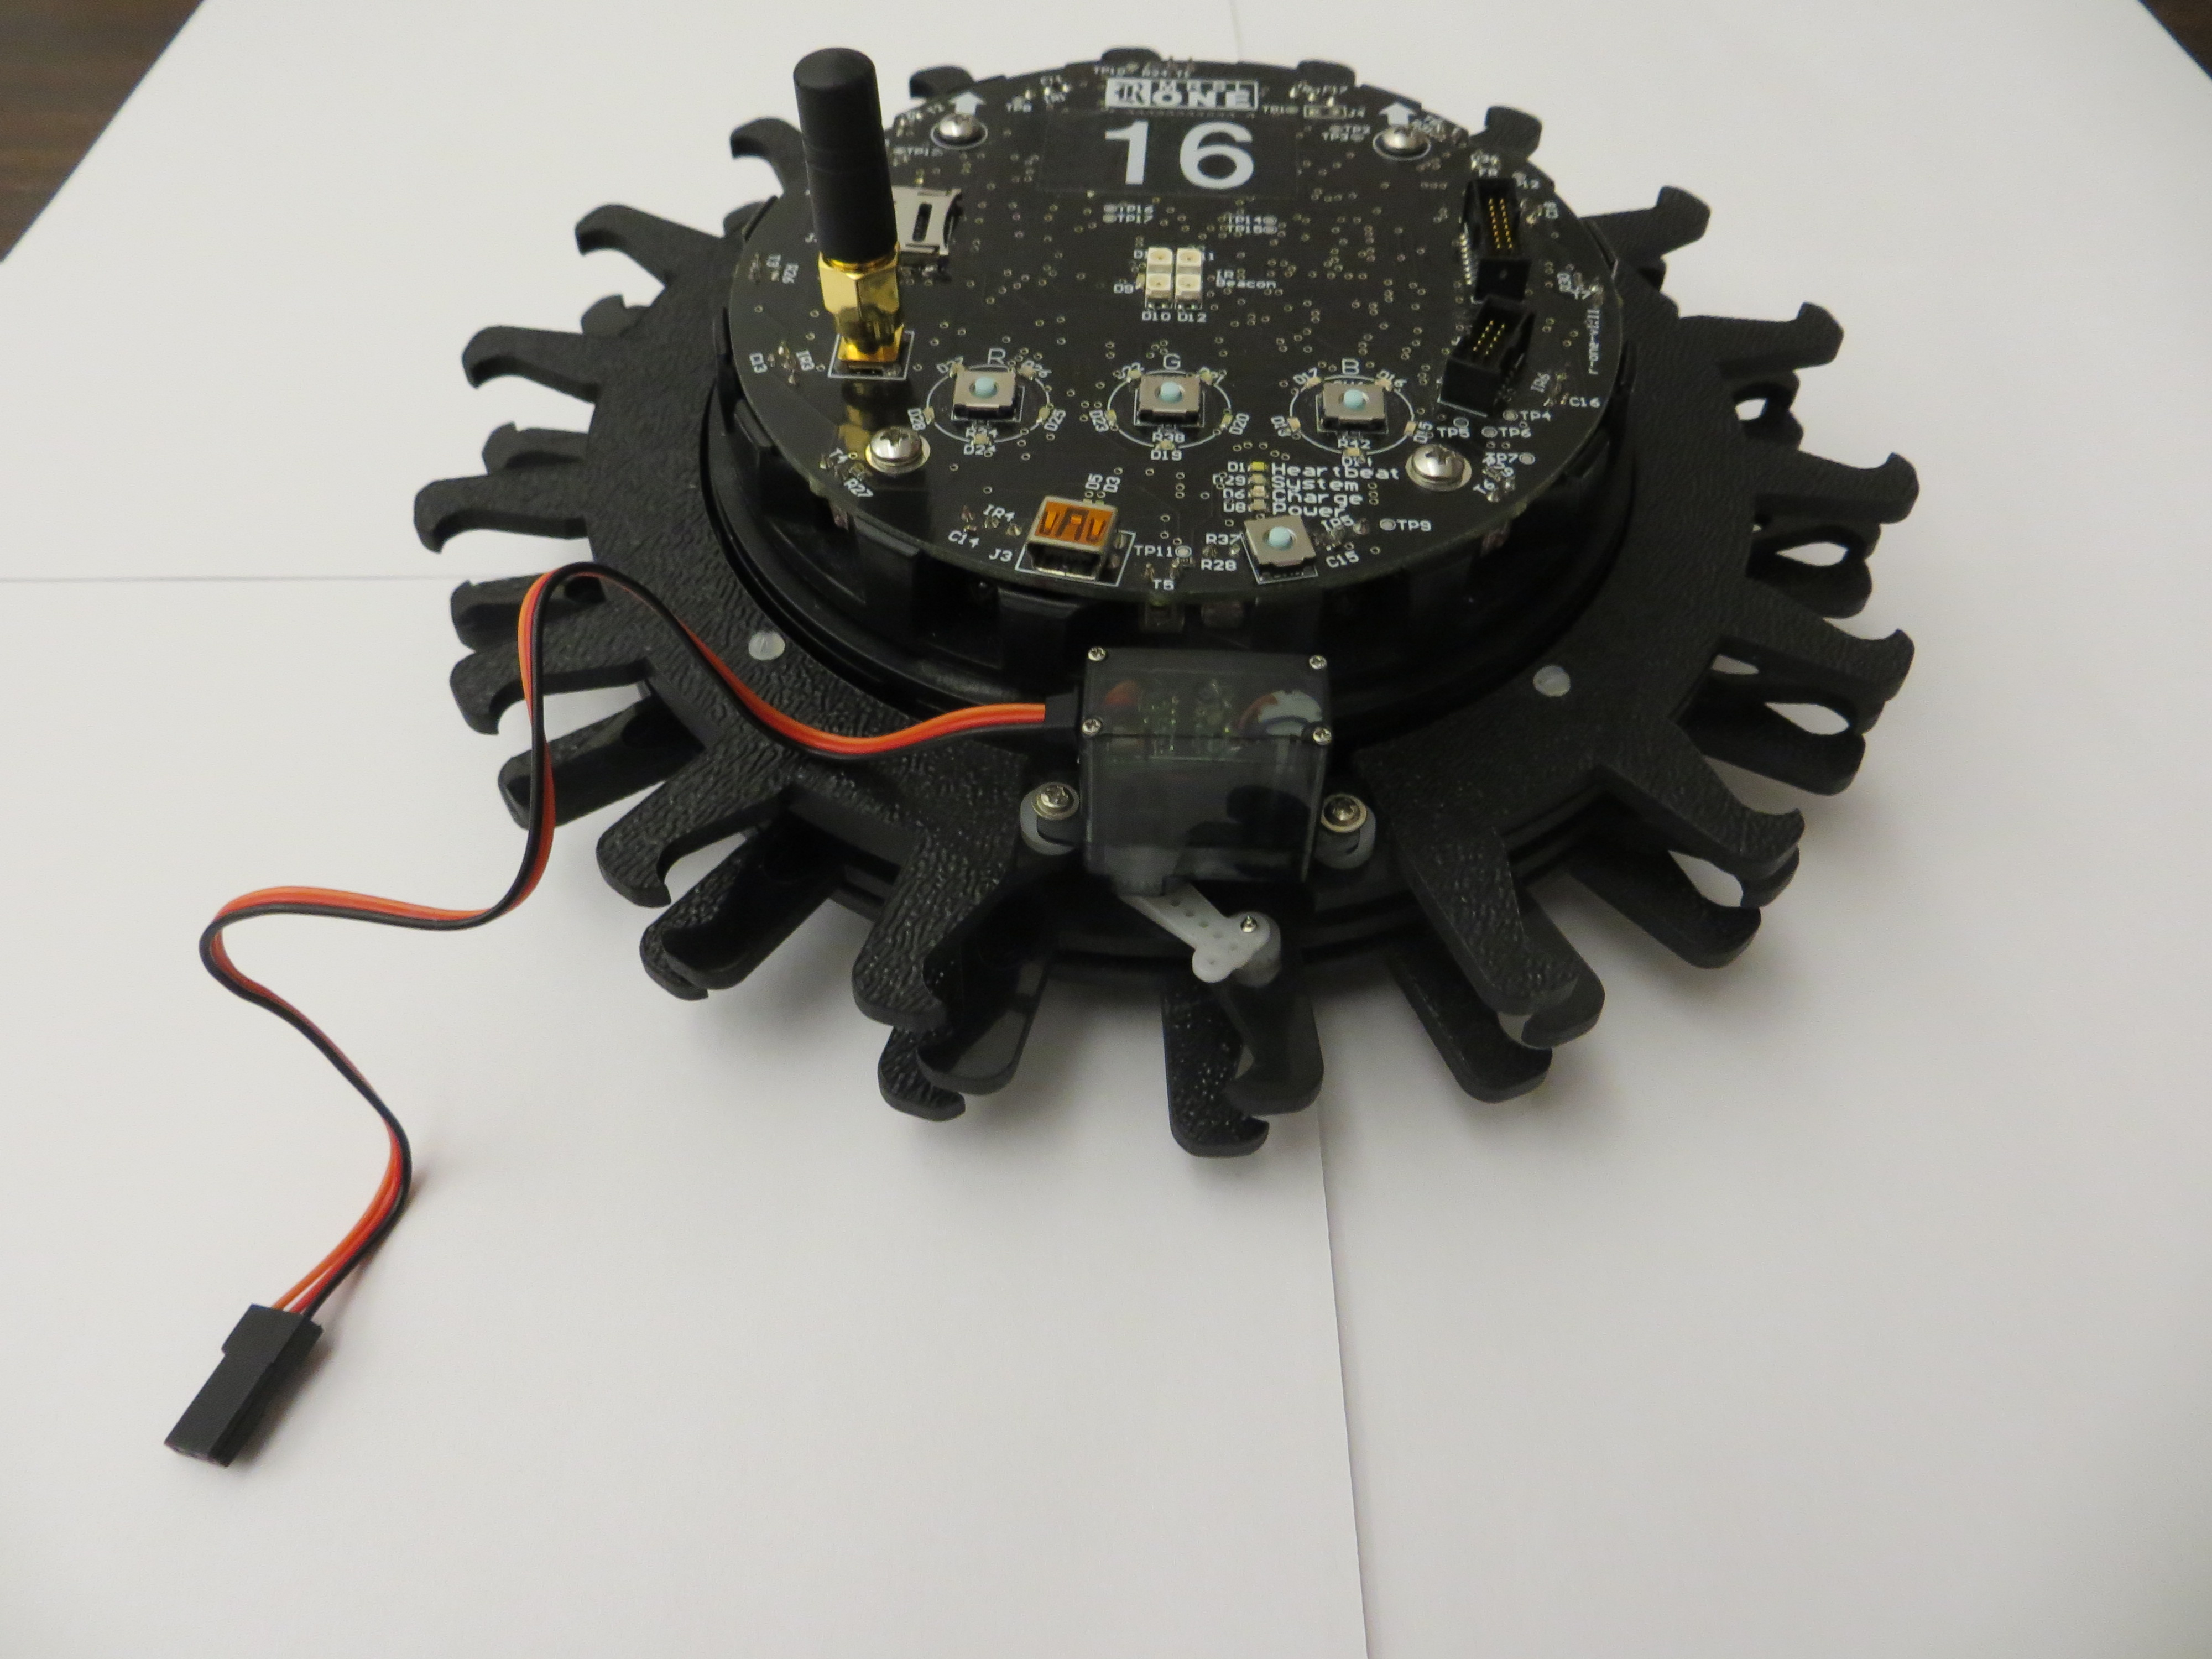
\includegraphics[width=.5\linewidth]{./Figs/back_closed}
\end{center}
\caption{}
\label{fig:back closed}
\end{figure}

There are many different components that go into the R-One Manipulator. A couple of them are just improvements over the last iteration of manipulator, the Velcro skirt, and others had to be specially designed for the purpose of the actuated manipulator. 

All of these components are laser cut from 1/8th inch ABS plastic. However, this is an option that can be reviewed for the best possible material to use. 

The servo used was pulled from the servo bin in the lab, and should be easily replaced. However, it may be beneficial for future use to find the smallest possible servo to minimize space requirements. 

\begin{figure}[h]
\begin{center}
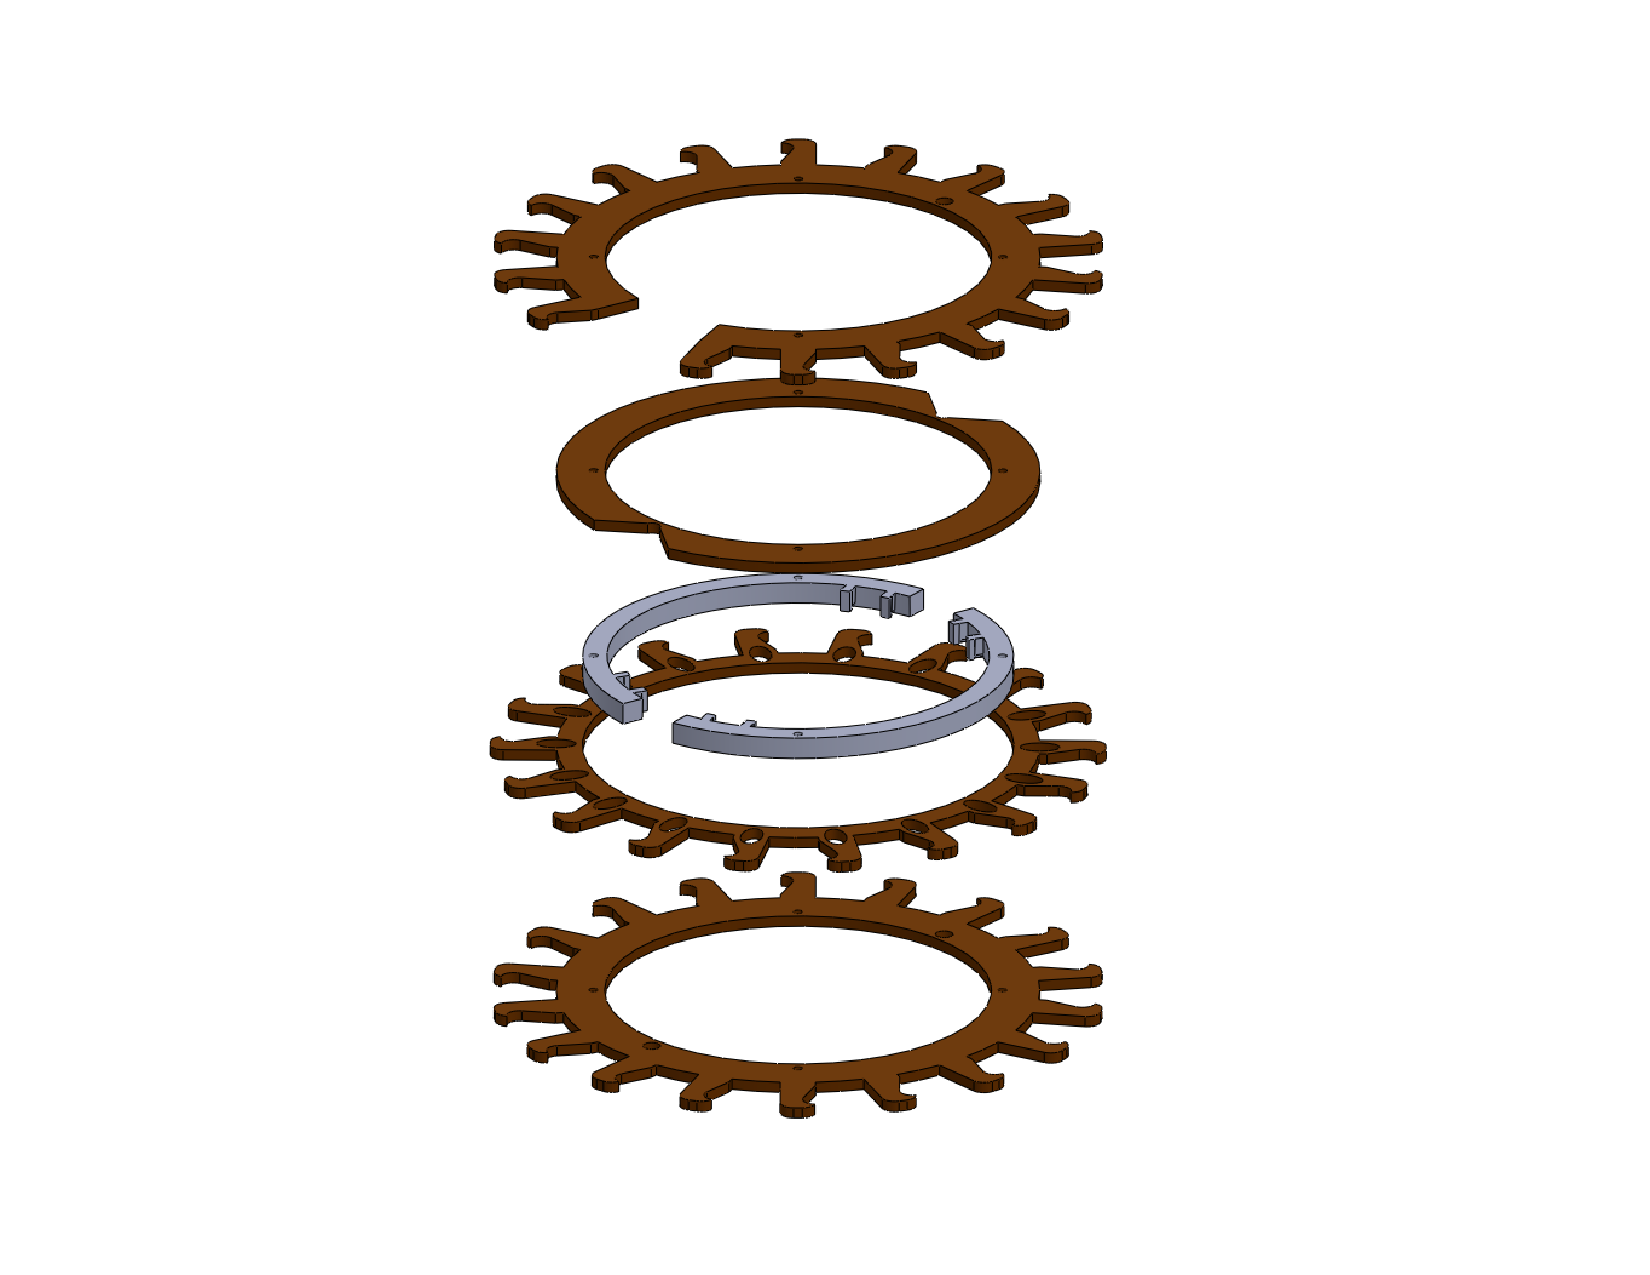
\includegraphics[width=.5\linewidth]{./Figs/final_assembly_explodedisometric.pdf}
\end{center}
\caption{An exploded view of the CAD model of the Actuated Manipulator}
\label{fig:explode}
\end{figure}

As we can see in Figure \ref{fig:explode} that there are five main laser cut components that make up this manipulator. We will start from the top and go to the bottom. The top is a stationary claw with a cutout to allow for the servo. Next is the spacer ring that has cutouts for the servo arm motion. On the prototype, we had to cut out more than the original laser cut-out to allow for the servo arm to rotate, so this will need to be adjusted in the SolidWorks model. Moving down, next comes the mounting clips, which should be already attached to the robot. On the screws, at this point, we installed some spacers (\#4 by 1/8th inch should suffice) Next on, comes the moving ring which fits around the spacers, to prevent lateral movement and isolate the radial movement. Finally, we attached the last stationary ring.
\bf{\sc{Note:}}Be sure to mount the rings so that the stationary claws are mounted in the same direction and a direction opposite to the moving claw.

All of these pieces are attached together with \#2-40x1.25in plastic slotted screws and \#2-40 washers, however the slotted screws can be replaced with metal hex head screws for added support.
\section{FURTHER RESEARCH}
\label{sec:Further}

Once we completed the design, building and research of the prototype actuated manipulator, we evaluated the potential issues that arose from what we had done. Below are listed a few options for improvements and/or directions to travel with the robot manipulator:
\begin{itemize}
\item Free Rotation
\begin{itemize}
\item Ideally, the whole apparatus needs to be free rotating similarly to the Velcro apparatuses so that the R-one can grab and object and turn to face any direction and then move.
\item Our prototype does not do this because of a concern of how to deal with the wires of having two counter-rotating servos. One way to solve this is to use a metal contact strip around the entirety of the robot that is in constant contact with the servo terminals in order to allow for free rotation.
\item Another option would be to run counter-rotation disks with the use of gears and mount the servo to the top or bottom.
\item This counter-rotation, however, forces problems of how to attach the manipulator to the robot. Having two disks rotate that cannot be connected to anything leads to a very flimsy or minimalist approach to design. The best solution to this we see is to continue using the bump skirt clips that have proven themselves from both the Velcro manipulator as well as our prototype actuated manipulator. 
\end{itemize}
\item The ring slot would work better if it was a slot, instead of an oval, this needs only a pin on an arm from the servo to drive it, instead of a large bulky screw.
\item The prototype requires a spacer between the moving ring and the bottom, stationary ring. This is evident in the video in the repository. Something thin with a cutout (like the ring the servo is mounted to) would probably work best.
\item One servo, clearly, works, however, using two may be better and provide a stronger grip. We didn't have time to experiment with this. 
\begin{itemize}
\item However, in order to prevent stripping/burning out of the servos, servo savers can be used. We were unable to find them small enough to fit for the application we require
\end{itemize}
\item Larger claws, or more spaced out claws would allow for gripping of larger objects and is a possibility for future adaptation. 
\item Making the claws thicker would help the robots grip one another, opening another area of research. 
\item An issue that we see is the design of the objects that are gripped by the robot, as they must have vertical, cylindrical shafts in order to be accurately grabbed by the robot. No known fix for this has been explored. It may just be that this is how things "in the robot world" must be constructed. 
\item Other ideas
\begin{itemize}
\item the moving ring could be an inverted gear (teeth on the inside) and the drive shaft comes through all layers and spins this. (it is also a possibility for part of the counter-rotating claw idea.)
\item explore different ideas for actuation using drive shafts, direct drives, and gears.
\end{itemize}
\item Incorporating a force sensor would be highly beneficial for the R-one manipulator project, because it would allow the R-one to detect when it has grabbed an object based from if the actuator has exceeded a certain force threshold, as long as the servo is not at its maximum wavelength. 
\end{itemize}

\section{APPENDIX}
\label{sec:Appendix}
The following pages include the SolidWorks drawings
of each piece required to assemble a the R-one actuated manipulator.

\end{document}

% % % %
%
%